%%%%%%%%%%%%%%%%%%%%%%%%%%%%%%%%%%%%%%%%%%%%%%%%%%%%%%%%%%%%%%%%%%%%%%%%%%%%%%%%
%2345678901234567890123456789012345678901234567890123456789012345678901234567890
%        1         2         3         4         5         6         7         8

\documentclass[letterpaper, 10 pt, conference]{ieeeconf}  % Comment this line out if you need a4paper

%\documentclass[a4paper, 10pt, conference]{ieeeconf}      % Use this line for a4 paper

\IEEEoverridecommandlockouts                              % This command is only needed if 
                                                          % you want to use the \thanks command

\overrideIEEEmargins                                      % Needed to meet printer requirements.

%In case you encounter the following error:
%Error 1010 The PDF file may be corrupt (unable to open PDF file) OR
%Error 1000 An error occurred while parsing a contents stream. Unable to analyze the PDF file.
%This is a known problem with pdfLaTeX conversion filter. The file cannot be opened with acrobat reader
%Please use one of the alternatives below to circumvent this error by uncommenting one or the other
%\pdfobjcompresslevel=0
%\pdfminorversion=4

% See the \addtolength command later in the file to balance the column lengths
% on the last page of the document

% The following packages can be found on http:\\www.ctan.org
%\usepackage{graphics} % for pdf, bitmapped graphics files
%\usepackage{epsfig} % for postscript graphics files
%\usepackage{mathptmx} % assumes new font selection scheme installed
%\usepackage{times} % assumes new font selection scheme installed
%\usepackage{amsmath} % assumes amsmath package installed
%\usepackage{amssymb}  % assumes amsmath package installed
\usepackage{amsmath}
\usepackage{graphicx}
\DeclareMathOperator*{\argmax}{arg\,max}
\DeclareMathOperator*{\argmin}{arg\,min}
\usepackage{amsfonts}
\usepackage{tabularx}
\usepackage{tabulary}

\title{\LARGE \bf
Traffic flow speed forecast on road graph with convolutional neural networks}


%\author{Nikolay G. Prokoptsev$^{1}$, Andrey E. Alekseenko$^{2}$, Yaroslav A. Kholodov$^{3}$}

\author{Nikolay Prokoptsev$^{1}$, Andrey Alekseenko$^{2}$, Yaroslav Kholodov$^{3}$% <-this % stops a space
\thanks{$^{1}$Innopolis University, 1 Universitetskaya st., Innopolis, Russia
        {\tt\small n.prokoptsev@innopolis.ru}}%
\thanks{$^{2}$Institute of Computer Aided Design of the Russian Academy of Sciences, 19/18 2-ya Brestskaya st.,  Moscow, Russia}%
\thanks{$^{3}$Innopolis University, 1 Universitetskaya st., Innopolis, Russia}
}

\begin{document}



\maketitle
\thispagestyle{empty}
\pagestyle{empty}


%%%%%%%%%%%%%%%%%%%%%%%%%%%%%%%%%%%%%%%%%%%%%%%%%%%%%%%%%%%%%%%%%%%%%%%%%%%%%%%%
\begin{abstract}

% The short-term prediction of road traffic condition is an important task of transportation modelling. A number of solutions exist - both model-driven and data driven had proven to be successful in capturing the dynamics of traffic flow. Neural networks, one of the prominent data-driven approaches, show promising performance in modelling the complexity of traffic flow. We present a neural network architecture for traffic flow prediction on a real-world road network graph. The model is based on the combination of a recurrent neural network and graph convolutional neural network. The resulting neural network was trained on raw data from traffic flow detectors from the US highway system and achieved lower prediction error than previously published models, such as Vector Auto Regression, LSTM and Graph Convolution GRU.
The short-term prediction of road traffic condition is an essential task of transportation modeling. A number of solutions exist -- both model-driven and data-driven -- that are successful in capturing the dynamics of traffic flow. Neural networks, one of the prominent data-driven approaches, show promising performance in modeling the complexity of traffic flow. We present a neural network architecture for traffic flow prediction on a real-world road network graph. The model is based on the combination of a recurrent neural network and a graph convolutional neural network. The resulting neural network was trained on raw data from traffic flow detectors from the US highway system and achieved lower prediction error than previously published models, such as Vector Auto Regression, LSTM and Graph Convolution GRU.
\end{abstract}

\begin{keywords}
Traffic flow prediction, Recurrent Neural Networks, Graph Convolutional Networks
\end{keywords}


%%%%%%%%%%%%%%%%%%%%%%%%%%%%%%%%%%%%%%%%%%%%%%%%%%%%%%%%%%%%%%%%%%%%%%%%%%%%%%%%
\section{Introduction}
Traffic flow and speed prediction are among the main tasks in the field of Intelligent Transportation Systems (ITS). A reliable and accurate system for traffic forecasting is essential for the efficient functioning of intelligent transport infrastructure --- and any modern city.

This problem can be formulated as a task of predicting some observable value, such as mean speed or intensity of the traffic flow, at a given node of the transport network based on current and historical data from nodes of the graph. In short-term forecasting problems, the prediction horizon typically does not exceed 1 hour.

Historically, two different approaches were used for this task. In the 1950s the first mathematical models of traffic flow emerged \cite{Richards1956, Lighthill1955}. These models try to describe traffic flow using the method of kinematic waves. As an alternative to model-based approach, the exponential increase in processing power of modern computer systems made data-driven approach possible.  Some examples of data-driven approach are ARIMA, KNN, Support Vector Regression, and Artificial Neural Networks.

The ARMA (Autoregressive moving average) model family played a key role in the development of this field of research. It includes such one-dimensional models as ARIMA \cite{Ahmed1979} and Seasonal ARIMA \cite{Williams2003}, which is a modification of ARIMA that makes use of seasonality in data. The main drawback of these models is they treat each sensor independently, ignoring the dependencies between neighboring sensors.

In the multivariate case, the most used model due to its simplicity is vector autoregression (VAR). It can take into the account spatial dependencies of the data. However, with the increase in the number of analyzed time series, the complexity of VAR-models grows quadratically, as it models dependencies of all sensors with all other sensors, which makes it difficult to apply them to large transport networks. The common limitation of this autoregressive models is that they model only linear dependencies between sensors which is not always the case.

Due to the stochastic and non-linear nature of the traffic data, researchers have paid much attention to nonparametric methods. The k-nearest neighbors (k-NN) method, a classic algorithm for regression, was proposed \cite{Davis1991} for short-term freeway traffic forecasting. However, its performance was on par with linear models and not better.

The Online Support Vector Regression (Online SVR) model \cite{Castro-Neto2009} has been successfully applied for predicting travel time in a transport network. This model allows updating the weights of the prediction function in real time using incremental learning. The method performed a bit better than baselines but significantly outperforms them in atypical non-recurring conditions, such as car accidents.

Researchers have long sought to use the potential of artificial neural networks (ANN) for traffic forecasting \cite{Jun2008}, but ANN with one hidden layer yielded worse results than SVR with the RBF kernel \cite{Lippi2013}.

Deep learning methods are widely and successfully used for a variety of tasks, such as machine translation, classification, and recognition of objects. Deep Belief Networks (DBN) have shown the potential of understanding the stochastic properties of traffic in unsupervised fashion \cite{Huang2014}. Stacked Autoencoders \cite{Lv2014} and Stacked Denoising Autoencoders \cite{Chen2016} were used to learn generic traffic flow features and find its latent properties. Such neural networks consider spatial and temporal  nonlinear correlations of traffic data, but they are difficult to train because of the fully connected layers in their architecture.

Recurrent Neural Networks (RNN) have become increasingly popular for time series and language modeling and achieved state-of-the-art results on popular datasets \cite{Greff2017}. Whereas feedforward networks only consider a fixed number of timesteps to predict the next one, recurrent neural networks can take into the account all preceding timesteps. Vanilla RNNs failed to scale to longtime dependencies due to vanishing gradient problem. This problem is addressed by Long Short-Term Memory (LSTM) \cite{Hochreiter1997} and Gate Recurrent Unit (GRU) \cite{Cho2014} networks. They catch not only short-term dependencies but also long-term ones. LSTM and GRU cell consists of several fully-connected components that capture spatiotemporal dependencies in data. The required complexity per timestep is $O(n^2)$, where $n$ is the number of detectors. 

In GRU and LSTM the use of hyperbolic tangent and the sigmoid activation functions results in gradient decay over layers, as these activation functions quickly saturate. Independent RNN \cite{Li2018} is a modification of RNN where neurons in each layer are independent of each other. Layers can be stacked to allow connection between neurons. Compared to LSTM this architecture allows to process much longer time series and construct deeper networks.

Convolutional Neural Networks (CNN) are the primary tool for modeling data with a spatial structure. They are particularly successful in extracting spatially local input patterns. These networks don’t suffer from the curse of dimensionality as they use space-invariant local filters. Moreover, stacking such filters allows capturing global features \cite{LeCun1998}. Vanilla CNNs work well with grid topology data, such as images, video, speech, but they are not designed for complex topologies such as graph.

Generalization of CNNs to graphs using tools from graph signal processing have been proposed \cite{Defferrard2016}. They approximate the graph Laplacian using Chebyshev expansion with free parameters that are learned during the training.  These networks employ fast local spectral filters to extract spatial properties in a neighborhood of a vertex of order $K$ with $O(K|\mathcal{E}|)$ complexity, where $|\mathcal{E}|$ is a number of edges. 

Graph Convolutional Networks \cite{kipf2017semi} simplify the previous method using an approximation of first-order Chebyshev expansion in Defferrard model. Each filter is applied only to the neighborhood of each node. In many experiments, this architecture surpasses other methods in terms of predicting accuracy.

The combination of recurrent neural networks and convolutional neural networks makes it possible to model spatially-temporal dependencies in data. The combination LSTM cell with convolution on a two-dimensional grid was proposed, where input-to-state and state-to-state transitions use convolution instead of matrix multiplication \cite{Shi2015}. Later it was extended \cite{Seo2016} to the case of the graph. Li et al. \cite{Li2017} proposed encoder-decoder architecture with Graph Convolutional GRU (GCGRU) which solves the noise accumulation problem.

\section{Methodology}
\subsection{Problem statement}
The value of flow, occupancy, and speed across all lanes at each detector station are aggregated and averaged for each 5-min interval for each detector station \cite{Chen2001}. This historical data of traffic flow from $N$ sensors at $M$ previous timesteps can be represented as the matrix $V=[v_1,v_2,...,v_M ]^T$ of size $M \times N $,  where $v_i$ is the vector of sensor readings at timestep $i$.

The connectivity between the sensors is defined by the undirected weighted graph of the transport network $\mathcal{G = (V, E, A)}$, where $\mathcal{V}$ is the set of vertices (sensors), $\mathcal{E}$ is the set of edges (roads), $\mathcal{A}$ is the weighted adjacency matrix of the graph that represents the connectivity of the sensors in the transport network.

Consequently, the problem of predicting the traffic flow in the road network can be formulated as follows:
\begin{equation}
v_{M + T} = \argmax{ p (v_{M + T}| v_1, v_2, ..., v_M, \mathcal{G})}
\end{equation}


\subsection{Proposed method}
The traffic flow detectors form a weighted graph, where we can define edge weights as a function of the distance between detectors. We assume that the influence between different parts of the road tends to decrease as the distance between them increases.

In this paper, we propose a new neural network architecture based on Independent RNN (IndRNN) \cite{Li2018} and Graph Convolutional Network (GCN) \cite{kipf2017semi}. We let the Graph Convolutional Network model spatial dependencies between sensors, while IndRNN is responsible for temporal dependencies. Each layer of the proposed model consists of an IndRNN, in which matrix multiplication is replaced with graph convolution followed by ReLU activation. This way, the convolution in each layer models spatial dependencies between adjacent nodes, while IndRNN models temporal dependencies of neurons independently. Stacking $k$ such layers will model spatiotemporal dependencies in $k$-th order neighborhood of each node.

\begin{figure}
    \centering
    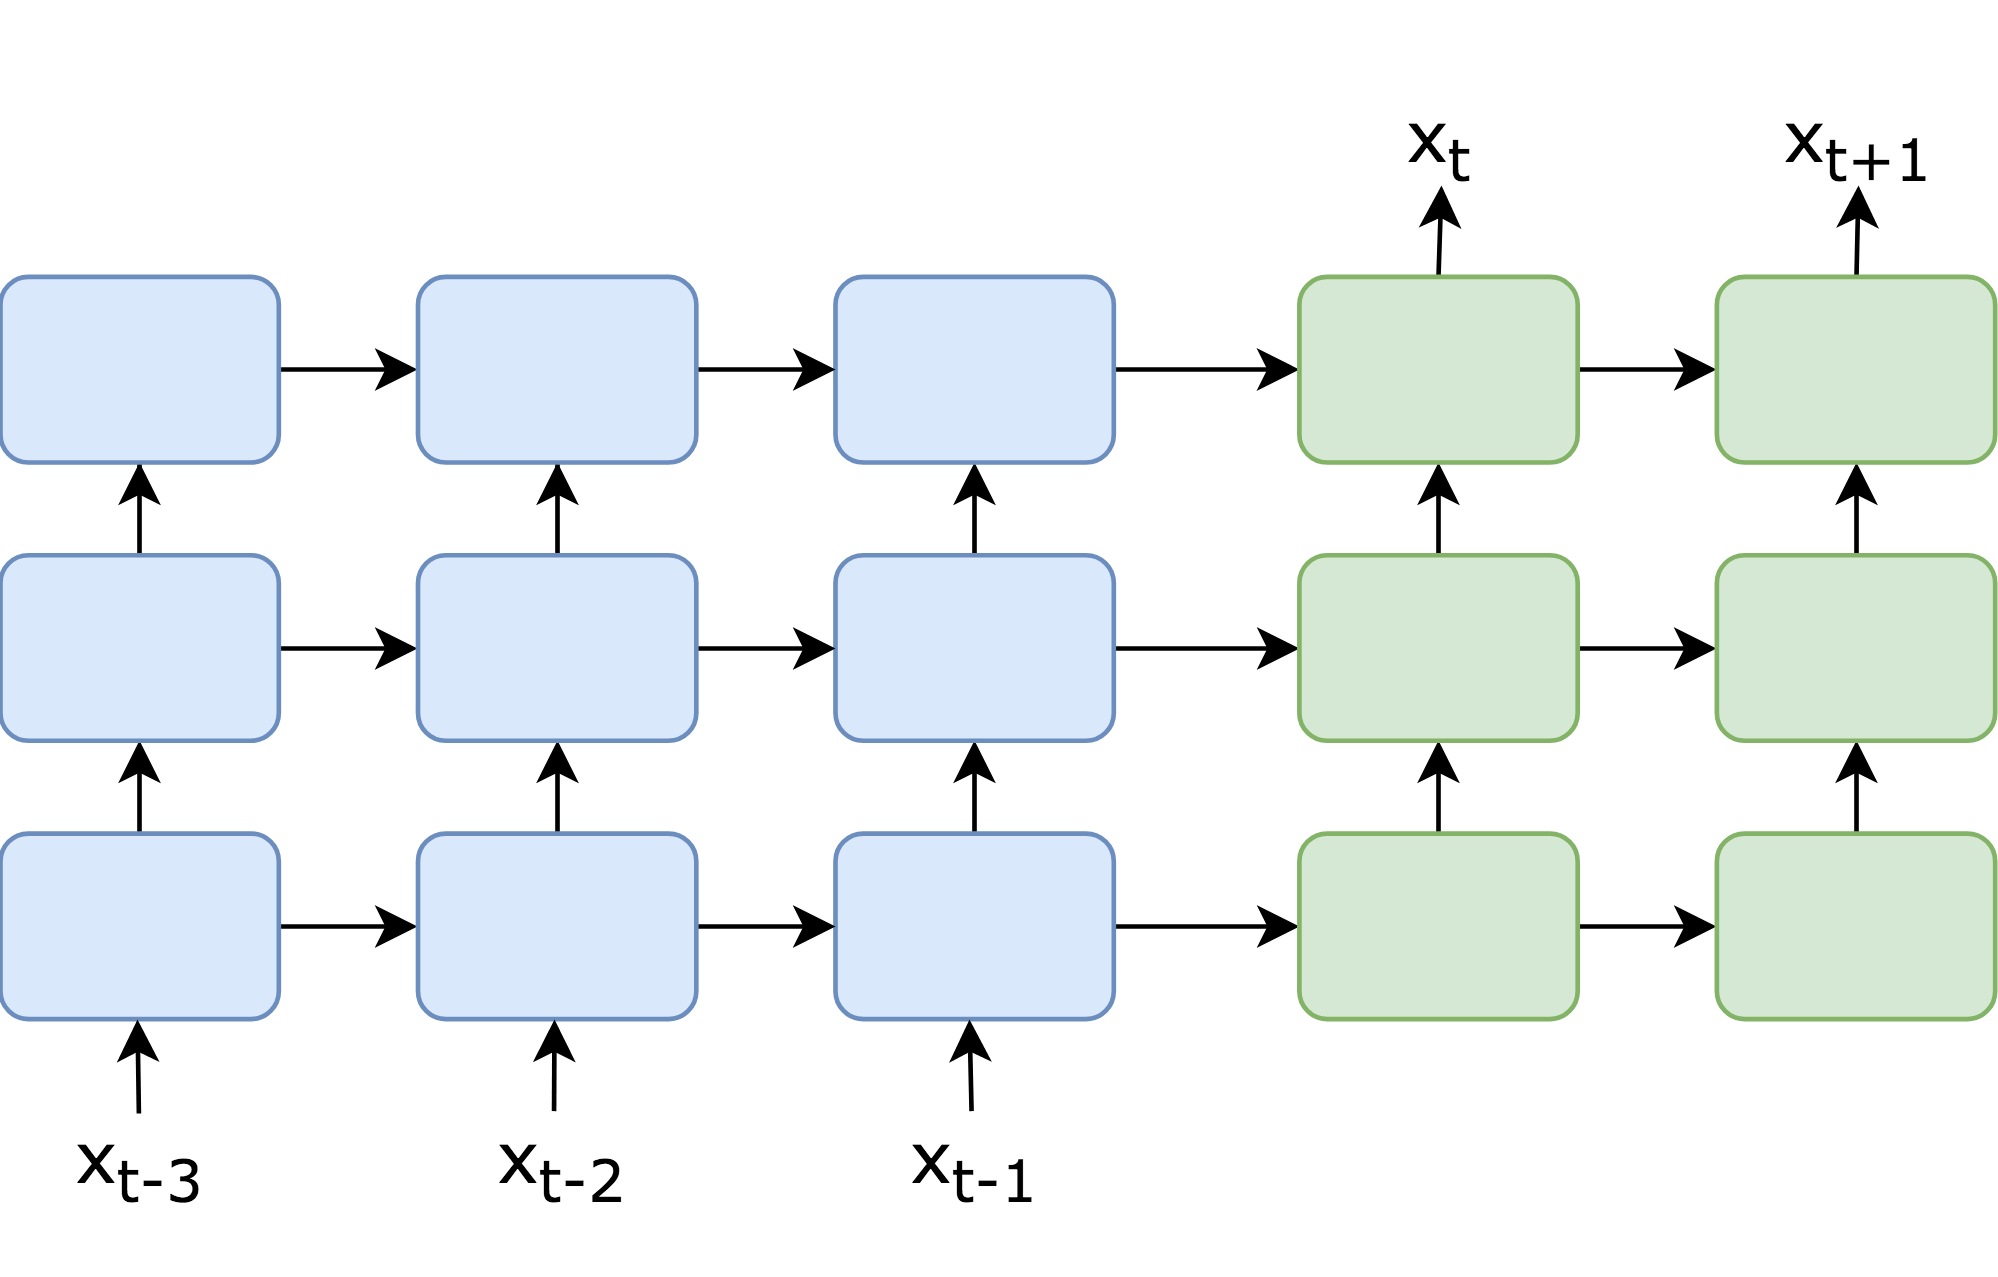
\includegraphics[width=0.4\textwidth]{encoder2.png}
    \caption{Encoder-decoder architecture for traffic flow forecasting. Blue cells represent the encoder, green cells represent the decoder.}
    \label{fig:encdec}
\end{figure}
Graph convolution for signal $ X \in \mathbb{R}^{N \times C} $ with $ C $ input channels is defined \cite{kipf2017semi} as follows:

\begin{equation}
Z = \widetilde{D}^{-\frac{1}{2}}\widetilde{A}\widetilde{D}^{-\frac{1}{2}}X\Theta,
\end{equation}
where  $Z \in \mathbb{R}^{N \times F}$ is the convolved signal matrix, $ \widetilde{D}_{ii}=\sum_j \widetilde{A}_{ij} $ is the diagonal node degree matrix, $ \widetilde{A} = A + I_N $, $ A $ is an adjacency matrix of graph, $I_N$ is an identity matrix, $ \Theta \in \mathbb{R}^{C \times F}$ is the matrix of filter parameters.

%We incorporate graph convolution into IndRNN cell, so 
Instead of processing inputs at each timestep with learned fully connected weight we use graph convolution.  We employ skip connections in our model to speed up training and make each layer model the residuals \cite{Kim2017}. To use skip connection in the first layer we have to upscale data, that has one feature map, to the same number of feature maps as are used for layer output. This transformation is performed with same transformation matrix for each detector. After the last layer, we have to downscale the number of feature maps to one. We tie the weights of matrix used for downscaling and upscaling to reduce the number of parameters.

Traditional models of traffic flow prediction, such as ARIMA and LSTM, suffer from noise propagation. This happens when we use predicted values from the previous step to predict the next ones. To deal with this problem we employ sequence to sequence model with encoder-decoder architecture \cite{Cho2014}, depicted on Figure \ref{fig:encdec}.

To train the sequence to sequence model we use teacher forcing. The training consists of maximizing the next value in the time series given the recurrent state and the ground truth value of the previous timestep. For inference, we replace the ground truth value with the predicted value. This behavior prevents neural network from adjusting to the accumulating noise during the training phase. To make a smooth transition from feeding true value to feeding generated value, we use scheduled sampling \cite{Bengio2015}.

\section{Experiments}
We used traffic data obtained from the Caltrans Performance Measurement System (PeMS) \cite{pems} District 4. The traffic speed averaged over 5-minute intervals was measured by 256 detectors on the Los Angeles highways for 4.5 months in 2016.  We divide data equally into train, validation and test set, 1.5 months each. To construct the detector graph, we define the adjacency matrix as follows:
\begin{equation}
    a_{ij} =
    \begin{cases}
        \exp\bigg(-\dfrac{d_{ij}^2}{\sigma^2}\bigg) & \text{if $ \exp\bigg(-\dfrac{d_{ij}^2}{\sigma^2}\bigg) > \varepsilon , i \neq j$,} \\
        0 & \text{otherwise,}
    \end{cases}
\end{equation}

where $d_{ij}$ is the distance between detectors, and $\sigma$ and $\varepsilon$ are parameters responsible for how sparse this matrix would be.

We compare our model with the following time series prediction baselines: 1) VAR, 2) Multilayered LSTM with fully connected input-to-state and state-to-state transitions (FC-LSTM) \cite{Sutskever2014}, 3) Graph Convolutional Gated Recurrent Unit (GCGRU).
All models are implemented in Tensorflow \cite{tensorflow2015-whitepaper} and are trained minimizing the mean square error with Adam optimizer \cite{Kingma2015}. We use batch size 32 and learning rate 0.001 and decrease it by the factor of 10 when performance on validation stops improving. The gradients are clipped by global norm 0.25. In addition, we perform standardization of inputs and fill missing values with zeros.

The VAR model is set to consider 12 lags. FC-LSTM consists of three layered LSTM network with tanh activation and hidden state of size 512. GCGRU is set to stack 2 recurrent graph convolution layers in decoder and encoder with each layer containing 64 GCGRU units. The maximum number of hops in graph convolution is set to 2.

Proposed model contains 7 residual layers of convolutional IndRNN with 64 channels in both encoder and decoder. It was set to consider 40 lags and predict 12 future timesteps. For scheduled sampling we employ sigmoid schedule, where we sample the true previous token at step $i$ with probability~$\epsilon_i$:
\begin{equation}
    \epsilon_i = k_0/(k_0+\exp(\max(0,i - k_1)/k_0)),
\end{equation}
where constants $k_0 \ge 1$ and $k_1 \ge 0$ depend on the expected speed of convergence. We we empirically found that $k_0 = 30$ and $k_1 = 5000$ leads to fastest convergence. 
 
We evaluate each approach for 3, 6 and 12 steps (15, 30, 60 minutes) ahead forecasting of a 5-minute average speed of each detector on the graph. For evaluation we use three metrics: mean absolute error (MAE), mean relative error (MAPE), and standard deviation (RMSE):
\begin{equation}
    \text{MAE} = \frac{1}{n}\sum_{t=1}^n |y_t - \hat{y}_t|
\end{equation}

\begin{equation}
    \text{MAPE} = \frac{1}{n}\sum_{t=1}^n \bigg|\dfrac{y_t - \hat{y}_t}{y_t}\bigg| * 100\%
\end{equation}

\begin{equation}
    \text{RMSE} = \sqrt{\frac{1}{n}\sum_{t=1}^n (y_t - \hat{y}_t)^2}
\end{equation}
where $n$ is a number of predictions, $y$ is \mbox{}the ground truth value of dependent variable (speed), $\hat{y}$ is the predicted value.

\newcolumntype{Z}[0]{>{\centering\arraybackslash}X}%
\begin{table}[]
    \centering
    \caption{Performance comparison of different approaches of traffic flow forecasting}
    \begin{tabularx}{0.47\textwidth}{|l|Z|Z|Z|}
    \hline
         & MAE (mph) & MAPE (\%) & RMSE (mph) \\ \hline\hline
        \multicolumn{4}{|c|}{15 minutes ahead} \\ \hline\hline
         VAR & 4.29 & 8.29 & 6.30  \\ \hline
         FC-LSTM & 2.92 & 6.22 & 5.40  \\ \hline
         GCGRU & 2.98 & 6.15 & 4.89  \\ \hline
         Proposed Method & 2.54 & 5.45 & 4.56 \\ \hline\hline
         \multicolumn{4}{|c|}{30 minutes ahead} \\ \hline\hline
         VAR & 5.72 & 11.15 & 8.51  \\ \hline
         FC-LSTM & 3.20 & 7.00 & 6.10  \\ \hline
         GCGRU & 3.67 & 7.57 & 5.97  \\ \hline
         Proposed Method & 2.78 & 6.14 & 5.10 \\ \hline\hline
         \multicolumn{4}{|c|}{60 minutes ahead} \\ \hline\hline
         VAR & 7.26 & 14.15 & 10.83  \\ \hline
         FC-LSTM & 3.52 & 7.86 & 6.87  \\ \hline
         GCGRU & 4.92 & 10.01 & 7.58  \\ \hline
         Proposed Method & 3.15 & 7.07 & 5.81 \\ \hline
    \end{tabularx}
    
    \label{tab:results_table}
\end{table}

Table \ref{tab:results_table} shows the comparison of different approaches for traffic flow prediction for 15, 30 and 60 minutes ahead forecast. 

\addtolength{\textheight}{-3.9cm}   % This command serves to balance the column lengths

The proposed method based on recurrent networks is more accurate than other methods. It shows noticeable gains (7\% to 15\%) in prediction performance and provides the best results considering all the metrics for all the horizons of the prediction. In terms of model complexity, the proposed network and GCGRU has $\sim10^5$ parameters each, while FC-LSTM has $\sim 10^7$.


\section{Conclusion}

In this article, we propose a data-driven approach for short-term traffic flow prediction. We present the neural network architecture capable of capturing the dynamic and complexity of traffic flow. The model is based on the combination of a recurrent neural network and a convolutional neural network on a graph. Encoder-decoder architecture paired with scheduled sampling successfully alleviates accumulating noise problem and allows predictions for multiple steps ahead.

The resulting neural network is trained on raw data from traffic flow sensors from the highway system around Los Angeles, USA, and the proposed model outperforms previous state-of-the-art methods, such as GCGRU, on a real traffic flow dataset by 7-15\%.

\section*{Acknowledgment}

This research has been supported by Russian Science Foundation (grant ID 14-11-00877).\\
The authors would also like to thank Google Cloud for providing access to GPUs that were used for training some of the models.


                                  % on the last page of the document manually. It shortens
                                  % the textheight of the last page by a suitable amount.
                                  % This command does not take effect until the next page
                                  % so it should come on the page before the last. Make
                                  % sure that you do not shorten the textheight too much.

%%%%%%%%%%%%%%%%%%%%%%%%%%%%%%%%%%%%%%%%%%%%%%%%%%%%%%%%%%%%%%%%%%%%%%%%%%%%%%%%



%%%%%%%%%%%%%%%%%%%%%%%%%%%%%%%%%%%%%%%%%%%%%%%%%%%%%%%%%%%%%%%%%%%%%%%%%%%%%%%%



%%%%%%%%%%%%%%%%%%%%%%%%%%%%%%%%%%%%%%%%%%%%%%%%%%%%%%%%%%%%%%%%%%%%%%%%%%%%%%%%
\bibliography{citations.bib} 
\bibliographystyle{ieeetr}

\end{document}
